%-------------------------------------------------------------------------------
% seq24_pattern_editor
%-------------------------------------------------------------------------------
%
% \file        seq24_pattern_editor.tex
% \library     Documents
% \author      Chris Ahlstrom
% \date        2015-07-19
% \update      2015-07-20
% \version     $Revision$
% \license     $XPC_GPL_LICENSE$
%
%     Provides the concepts.
%
%-------------------------------------------------------------------------------

\section{Pattern Editor}
\label{sec:seq24_pattern_editor}

   The \textsl{Seq24 Pattern Editor} is used to edit a pattern.

   TODO

\begin{figure}[H]
   \centering 
   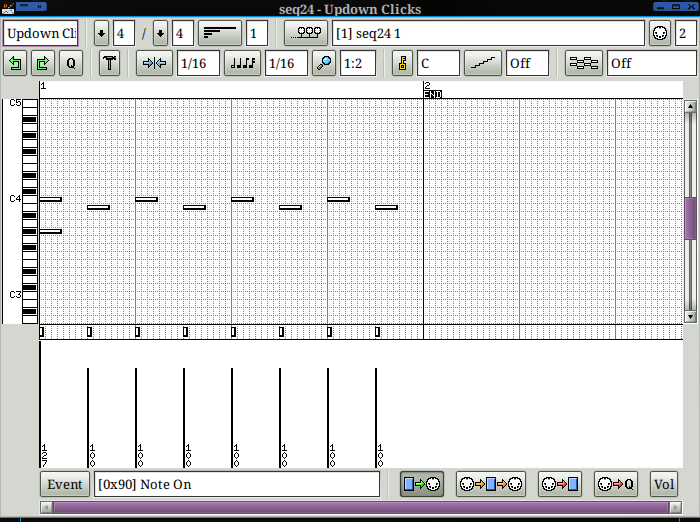
\includegraphics[scale=0.75]{pattern/pattern-edit-window.png}
   \caption{Pattern Edit Window}
   \label{fig:pattern_edit_window}
\end{figure}

   This dialog is quite complex.
   For exposition, we break it into a first panel, a second panel, a
   bottom panel, and a piano-roll/events section.

   \begin{enumber}
      \item \textbf{First Panel}
      \item \textbf{Second Panel}
      \item \textbf{Piano-Roll/Events Panel}
      \item \textbf{Bottm Panel}
   \end{enumber}

\subsection{Pattern Editor, First Panel}
\label{subsec:seq24_pattern_editor_first}

   The top bar of the pattern (sequence) editor lets you change the name of
   the pattern, the time signature of the piece, how long the loop is, and
   some other configuration items.

\begin{figure}[H]
   \centering 
   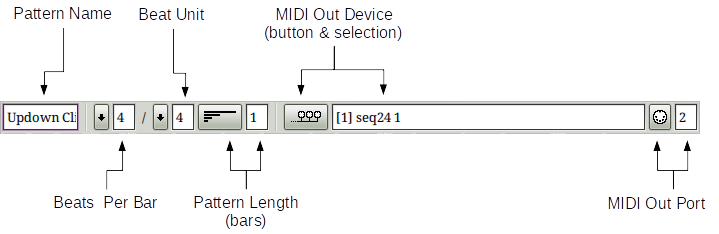
\includegraphics[scale=0.75]{pattern/pattern-edit-first-panel-items.png}
   \caption{Pattern Editor, First Panel Items}
   \label{fig:pattern_editor_first_panel_items}
\end{figure}

   \begin{enumber}
      \item \textbf{Pattern Name}
      \item \textbf{Beats Per Bar}
      \item \textbf{Beat Unit}
      \item \textbf{Pattern Length}
      \item \textbf{MIDI Out Device}
      \item \textbf{MIDI Out Port}
   \end{enumber}

   \setcounter{ItemCounter}{0}      % Reset the ItemCounter for this list.

   \itempar{Pattern Name}{pattern!name}
   Provides the name of the pattern.
   This name should be short and memorable.
   It is displayed in the Patterns window.

   \itempar{Beats Per Bar}{pattern!beats/bar}
   Part of the time signature, and specifies the number of beat units per bar.
   The possible values range from 1 to 16.

   \itempar{Beat Unit}{pattern!beat unit}
   Part of the time signature, and specifies the size of the beat unit:
   1 for whole notes; 2 for half notes; 4 for quarter notes; 8 for eight notes;
   and 16 for sixteenth notes.

   \itempar{Pattern Length}{pattern!progress}
   Sets the length of the current pattern, in measures.
   The possible values range from 1 to 16, then 32, and 64.

   \textsl{(It would sure be nice to have a value that represents
   "indefinite", so that the loop or pattern would be more like track,
   and perhaps not be repeatable.)}

   \itempar{MIDI Out Device}{pattern!midi out device}
   This setting specifies one of the 16 MIDI output busses provided by
   \textsl{Seq24}.  The settings look a lot like
   \figureref{fig:pattern_window_right_click_midi_bus}.

   \itempar{MIDI OUT Port}{pattern!midi out port}
   This settings select the MIDI output channel, or port.
   The possible values range from 1 to 16.

\subsection{Pattern Editor, Second Panel}
\label{subsec:seq24_pattern_editor_second}

   The second panel of the pattern editor provides a number of additional
   settings.

\begin{figure}[H]
   \centering 
   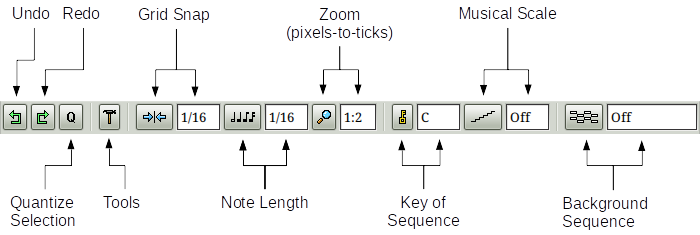
\includegraphics[scale=0.75]{pattern/pattern-edit-second-panel-items.png}
   \caption{Pattern Editor, Second Panel Items}
   \label{fig:pattern_editor_main_panel_items}
\end{figure}

   \begin{enumber}
      \item \textbf{Undo}
      \item \textbf{Redo}
      \item \textbf{Quantize Selection}
      \item \textbf{Tools}
      \item \textbf{Grid Snap}
      \item \textbf{Note Length}
      \item \textbf{Zoom}
      \item \textbf{Key of Sequence}
      \item \textbf{Musical Scale}
      \item \textbf{Background Sequence}
   \end{enumber}

   \setcounter{ItemCounter}{0}      % Reset the ItemCounter for this list.

   \itempar{Undo}{pattern!undo}
   The Undo button will roll back any changes to the pattern from this session.

   \itempar{Redo}{pattern!redo}
   The Redo button will restore any undone changes to the pattern from this
   session.

   \itempar{Quantize Selection}{pattern!quantize}
   Pressing this button will quantize the selected events, presumable as per
   the \textbf{Grid Snap} setting.

   \itempar{Tools}{pattern!tools}
   This button brings up a nested menu of tools for modifying selected
   events and notes.

\begin{figure}[H]
   \centering 
   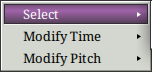
\includegraphics[scale=0.75]{pattern/tools-first-menu.png}
   \caption{Tools Context Menu}
   \label{fig:pattern_editor_tools_first_menu}
\end{figure}

   \begin{enumber}
      \item \textbf{Select}
      \item \textbf{Modify Time}
      \item \textbf{Modify Pitch}
   \end{enumber}

   \textbf{Select} provides two sets of selections for notes:
   \textbf{All Notes}, which selects all notes in the pattern;
   \textbf{Inverse Notes}, which inverts the selection of notes.

   Note that the left mouse button also lets one select multiple events and
   notes.

   \textbf{Modify Time} offers two ways to tweak the timing of the selected
   note:
   \textbf{Quantize Selected Notes}, which quantizes the selected notes,
   presumably the same way as the \textbf{Quantize} ("\textbf{Q}") button;
   \textbf{Tighten Selected Notes}, which presumably is a less strict form
   of quantization.  (Need more information).

   \textbf{Modify Pitch} has only one entry, \textbf{Transpose Selected},
   which brings up the following sub-menu:

\begin{figure}[H]
   \centering 
   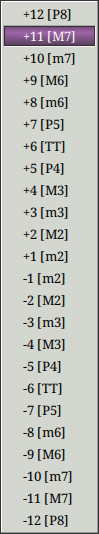
\includegraphics[scale=0.75]{pattern/tools-transpose-selected-menu.png}
   \caption{Tools Transpose Selected Values}
   \label{fig:pattern_editor_tools_transpose_selected_menu}
\end{figure}

   \itempar{Grid Snap}{pattern!grid snap}
   Grid snap selects where the notes will be drawn.
   The following values are supported:
   1, 1/2, 1/4, 1/8, 1/16, 1/32, 1/64, and 1/128.
   Additional values are also supported:
   1/3, 1/6, 1/12/, 1/24, 1/48, 1/96, and 1/192.

   \itempar{Note Length}{pattern!note length}
   Note Length determines what size they will be.
   Like the \textbf{Grid Snap} values,
   the following values are supported:
   1, 1/2, 1/4, 1/8, 1/16, 1/32, 1/64, and 1/128.
   Additional values are also supported:
   1/3, 1/6, 1/12/, 1/24, 1/48, 1/96, and 1/192.

   \itempar{Zoom}{pattern!zoom}
   Zoom is the relation between MIDI pixels and ticks, written as
   "pixels:ticks.
   For example, 1:4 = 4 ticks per pixel.
   Supported values are 1:1, 1:2, 1:4, 1:8, 1:16, and 1:32.

   \itempar{Key of Sequence}{pattern!key}
   Selects the desired key for the pattern.  The following scales are
   supported:  C, C\#, D, D\#, E, F, F\#, G, G\#, A, A\#, and B.

   \itempar{Musical Scale}{pattern!scale}
   Selects the desired scale for the pattern.
   Only the following values are supported: Off, Major, and Minor.

   One can select which \textbf{Musical Scale} and
   \textbf{Key} the piece is in,
   and \textsl{Seq24} will grey out those keys on the piano-roll that
   are not in the key.

   \itempar{Background Sequence}{pattern!background sequence}
   One can select another pattern to draw on the background to help with
   writing corresponding parts.
   The button brings up a small menu with values of \textbf{Off} and
   \textbf{[0]}.  Presumably, the 0 is a set number.  Under that entry, a
   menu like the following appears.

\begin{figure}[H]
   \centering 
   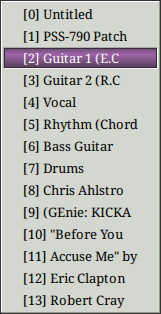
\includegraphics[scale=0.75]{pattern/background-sequence-menu.png}
   \caption{Sample Background Sequence Values}
   \label{fig:pattern_editor_background_sequence_menu}
\end{figure}

\subsection{Pattern Editor, Piano Roll}
\label{subsec:seq24_pattern_editor_piano_roll}

   The piano roll is the heart of the pattern (loop, sequence) editor.
   It is a bit different in style than other editors.

\begin{figure}[H]
   \centering 
   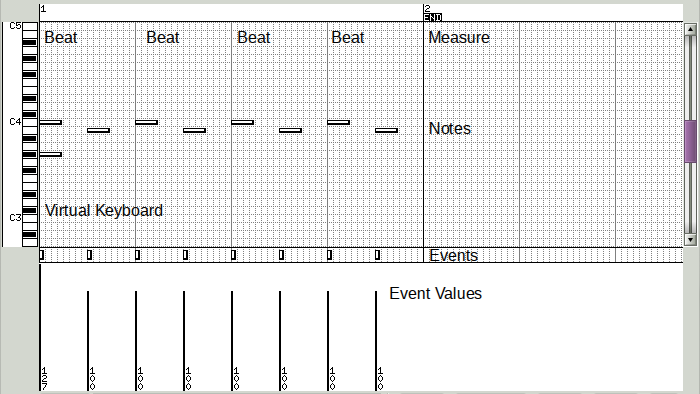
\includegraphics[scale=0.75]{pattern/pattern-edit-piano-roll-items.png}
   \caption{Pattern Editor, Piano Roll Items}
   \label{fig:pattern_editor_piano_roll_items}
\end{figure}

   \begin{enumber}
      \item \textbf{Beat}
      \item \textbf{Measure}
      \item \textbf{Virtual Keyboard}
      \item \textbf{Notes}
      \item \textbf{Events}
      \item \textbf{Event Values}
   \end{enumber}

   \setcounter{ItemCounter}{0}      % Reset the ItemCounter for this list.

   \itempar{Beat}{piano roll!beat}
   The light vertical lines represent the beats defined by the configuration
   for the pattern.

   \itempar{Measure}{piano roll!measure}
   The heavy vertical lines represent the measures defined by the configuration
   for the pattern.  Also note that the end of the pattern occurs at a
   measure, and is marked by a blocky \textbf{END} marker.

   \itempar{Virtual Keyboard}{piano roll!virtual keyboard}

   \itempar{Notes}{piano roll!notes}

   \itempar{Events}{piano roll!events}

   \itempar{Event Values}{piano roll!event values}

\begin{figure}[H]
   \centering 
   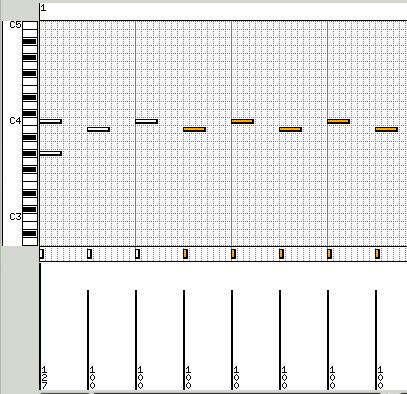
\includegraphics[scale=0.75]{pattern/pattern-edit-selected-events.png}
   \caption{Piano Roll, Selected Notes and Events}
   \label{fig:pattern_editor_selected_events}
\end{figure}

   TODO

\subsection{Pattern Editor, Bottom Panel}
\label{subsec:seq24_pattern_editor_bottom}

   TODO

\begin{figure}[H]
   \centering 
   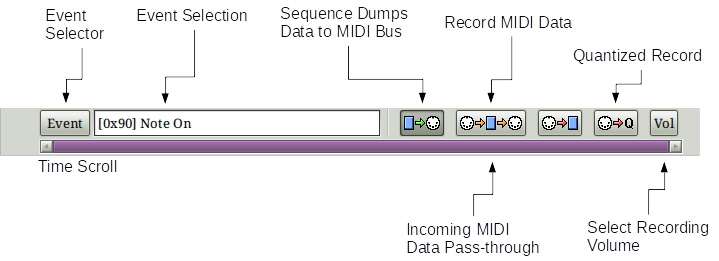
\includegraphics[scale=0.75]{pattern/pattern-edit-bottom-panel-items.png}
   \caption{Pattern Editor, Bottom Panel Items}
   \label{fig:pattern_editor_bottom_panel_items}
\end{figure}

   TODO


%-------------------------------------------------------------------------------
% vim: ts=3 sw=3 et ft=tex
%-------------------------------------------------------------------------------
